\documentclass[a4paper,twoside]{book}

\emergencystretch=1em
\usepackage[utf8]{inputenc}
\usepackage[english]{babel}
\usepackage{fontspec}
\usepackage{graphicx}
\renewcommand{\thefigure}{\thesection.\arabic{figure}}
\usepackage{hyperref}
\usepackage{multirow}
\usepackage[absolute,overlay,showboxes]{textpos}
\usepackage{etoolbox}
\usepackage{longtable}
\usepackage{tikz}
\usepackage{lilyglyphs}
\usepackage{tabularx}
\usepackage{pgfplots}
\usepackage{circuitikz}
\usepackage{minted}
\usepackage{glossaries}
\usepackage{makeidx}
\usepackage{expl3}
\usepackage{chngcntr}
\usepackage{svg}
\usepackage{subfiles}
\usepackage[printonlyused,withpage]{acronym}

\usepackage[backend=bibtex]{biblatex}
\addbibresource{references.bib}

%%%%%%%%%%%%%%%%%%%%%%%%%%%%%%%%%%%%%%%%%%%%%%%%%%%%%%%%%%%%%%%%%%%%%%%%%%%%%%%%
\setmainfont{Liberation Serif}
\setmonofont{Liberation Mono}

\makeindex
\makeglossaries

\urlstyle{same}

\graphicspath{ {images/} {../../../images/} {../../../out/src/common/} }

%% \documentclass[../main.tex]{subfiles}
%% \usepackage{svg}
%% \graphicspath{{\subfix{../images/}}}
%% \begin{document}

\newcounter{example-counter}
\setcounter{example-counter}{1}

%% This procedure adds the "Example" block to the text.
\newcommand{\example}[1]{
  \vspace{8pt}
  \begin{tabularx}{\textwidth}{m{1cm} m{9cm}}
    \includesvg[width=1.25cm]{the-noun-project/request-mirrored}
    & \textbf{Пример \arabic{example-counter}}: #1 \\
  \end{tabularx}
  \addtocounter{example-counter}{1}
}

\newcounter{experiment-counter}
\setcounter{experiment-counter}{1}

%% This procedure adds the "Experiment" block to the text.
\newcommand{\experiment}[2]{
  \vspace{8pt}
  \begin{tabularx}{\textwidth}{m{.15\textwidth}X m{.85\textwidth-4}X}
    \includesvg[width=1cm]{the-noun-project/flask}
    & \textbf{Эксперимент №\arabic{experiment-counter}:} #2 \\
  \end{tabularx}
  \addtocounter{experiment-counter}{1}
}

\newcommand{\note}[1]{
  \vspace{8pt}
  \begin{tabularx}{\textwidth}{m{1cm} m{9cm}}
    \includesvg[width=1cm]{the-noun-project/note}
    & \textbf{Примечание:} #1 \\
  \end{tabularx}
}

\newcommand{\hotkey}[1]{
  \texttt{#1}
}

%% This procedure allows to insert a music note.
%% Syntax:
%%   \musicnote{<octave>}{<note-name>}{<frequency>}
\newcommand{\musicnote}[3]{
  &
  \ifstrequal{#2}{C}{До   & C#1}{}
  \ifstrequal{#2}{D}{Ре   & D#1}{}
  \ifstrequal{#2}{E}{Ми   & E#1}{}
  \ifstrequal{#2}{F}{Фа   & F#1}{}
  \ifstrequal{#2}{G}{Соль & G#1}{}
  \ifstrequal{#2}{A}{Ля   & A#1}{}
  \ifstrequal{#2}{B}{Си   & B#1 (H#1)}{}
  & #3 \\
}

%% Taken from:
%%   <https://tex.stackexchange.com/questions/184923/how-to-include-a-second-file-only-if-environment-variable-is-set>
\newcommand{\newgetenv}[2][]{%
 \CatchFileEdef{\temp}{"|kpsewhich --var-value #2"}{\endlinechar=-1\relax}%
 \if\relax\detokenize{#1}\relax\temp\else\edef#1{\temp}\fi%
}%

\newcommand\esymbol[1]{%
  \begin{circuitikz}%
    \draw (0,0) to [#1] (1,0);%
  \end{circuitikz}%
}

\newcommand*{\soundWaveIcon}[0]{%
  
\begin{tikzpicture}
    \draw[black, fill=black] (0, 0) circle (.25mm);
    \draw (.5mm, 0.7mm) arc (45:-45:1mm);
    \draw (1mm, 1mm) arc (45:-45:1.5mm);
    \draw (1.5mm, 1.3mm) arc (45:-45:2mm);
  \end{tikzpicture}%
}

%% \end{document}

\newcommand{\figureSoundGraph}[1]{
  \begin{figure}[H]
    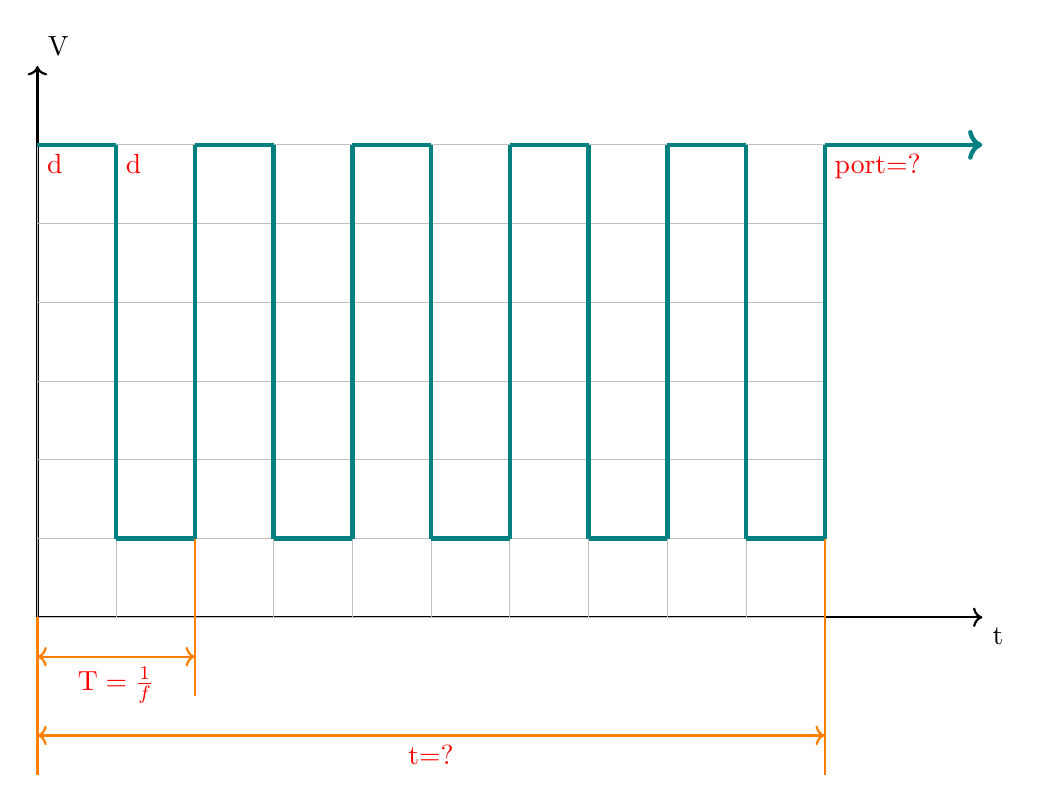
\begin{tikzpicture}
      \draw[thick, ->] (0, 0) -- (12, 0) node[anchor=north west] {t};
      \draw[thick, ->] (0, 0) -- (0,  7) node[anchor=south west] {V};
      \draw[lightgray] (0, 0) grid (10, 6);
      \foreach \x in {0, 2, ..., 8} {
        \draw[ultra thick, teal] (\x, 6) -- (\x + 1, 6);
        \draw[ultra thick, teal] (\x + 1, 6) -- (\x + 1, 1);
        \draw[ultra thick, teal] (\x + 1, 1) -- (\x + 2, 1);
        \draw[ultra thick, teal] (\x + 2, 1) -- (\x + 2, 6);
      }
      \draw[ultra thick, teal, ->] (10, 6) -- (12, 6);
      \draw[orange] (10, 6) node[anchor=north west, red] {port=?};
      \draw[orange] (0, 6) node[anchor=north west, red] {d};
      \draw[orange] (1, 6) node[anchor=north west, red] {d};
      \draw[thick, orange] (0,  0) -- (0,   -2);
      \draw[thick, orange] (2,  1) -- (2,   -1);
      \draw[thick, orange] (10, 1) -- (10,  -2);
      \draw[thick, orange, <->] (0, -0.5)
      -- (2,  -0.5) node[midway, below, red] {$\mbox{T} = \frac{1}{f}$};
      \draw[thick, orange, <->] (0, -1.5)
      -- (10,  -1.5) node[midway, below, red] {t=?};
    \end{tikzpicture}
    \caption{#1}
    \label{fig:sound-graph}
  \end{figure}
}

\newcommand{\figurePWMGraph}[2]{
  \def\lang{\detokenize{#1}}
  \def\langRu{\detokenize{ru}}
  \def\langEn{\detokenize{en}}
  \def\figureCaption{XXX: No translation.}
  \def\figureUnit{$\mu\mbox{s}$}
  \ifx \lang\langRu
  \def\figureCaption{
    Графическое отображение процесса генерации ШИМ-сигнала.
  }
  \def\figureUnit{мкс}
  \fi
  \ifx \lang\langEn
  \def\figureCaption{
    A graphical representation of the PWM signal generation.
  }
  \def\figureUnit{$\mu\mbox{s}$}
  \fi
  \begin{figure}[ht]
    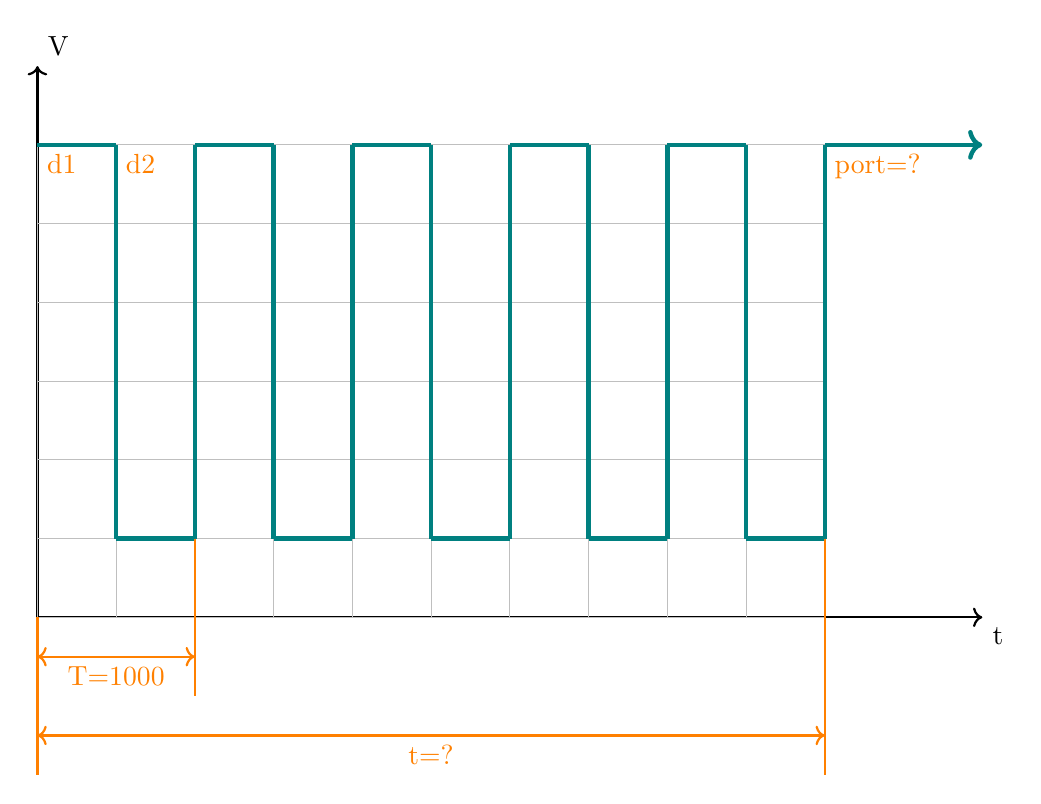
\begin{tikzpicture}
      \draw[thick, ->] (0, 0) -- (12, 0) node[anchor=north west] {t};
      \draw[thick, ->] (0, 0) -- (0,  7) node[anchor=south west] {V};
      \draw[lightgray] (0, 0) grid (10, 6);
      \foreach \x in {0, 2, ..., 8} {
        \draw[ultra thick, teal] (\x, 6) -- (\x + 1, 6);
        \draw[ultra thick, teal] (\x + 1, 6) -- (\x + 1, 1);
        \draw[ultra thick, teal] (\x + 1, 1) -- (\x + 2, 1);
        \draw[ultra thick, teal] (\x + 2, 1) -- (\x + 2, 6);
      }
      \draw[ultra thick, teal, ->] (10, 6) -- (12, 6);
      \draw[orange] (10, 6) node[anchor=north west] {port=?};
      \draw[orange] (0, 6) node[anchor=north west] {d1};
      \draw[orange] (1, 6) node[anchor=north west] {d2};
      \draw[thick, orange] (0,  0) -- (0,   -2);
      \draw[thick, orange] (2,  1) -- (2,   -1);
      \draw[thick, orange] (10, 1) -- (10,  -2);
      \draw[thick, orange, <->] (0, -0.5) -- (2,  -0.5)  node[midway, below] {T=1000 \figureUnit};
      \draw[thick, orange, <->] (0, -1.5) -- (10,  -1.5) node[midway, below] {t=?};
    \end{tikzpicture}
    \caption{\figureCaption}
    \label{fig:pwm-graph}
  \end{figure}
}

\newcommand{\figureADC}[1]{
  \def\lang{\detokenize{#1}}
  \def\langRu{\detokenize{ru}}
  \def\langEn{en}
  \def\figureCaption{XXX: No translation.}
  \ifx \lang\langRu
  \def\figureCaption{
    Схематическое изображение 10-битного аналогово-цифрового
    преобразователя (АЦП.)
  }
  \fi
  \if \lang\langEn
  \def\figureCaption{
    Schematic depiction of the 10-bit analog-to-digital converted (ADC.)
  }
  \fi
  \begin{figure}[ht]
    \centering
    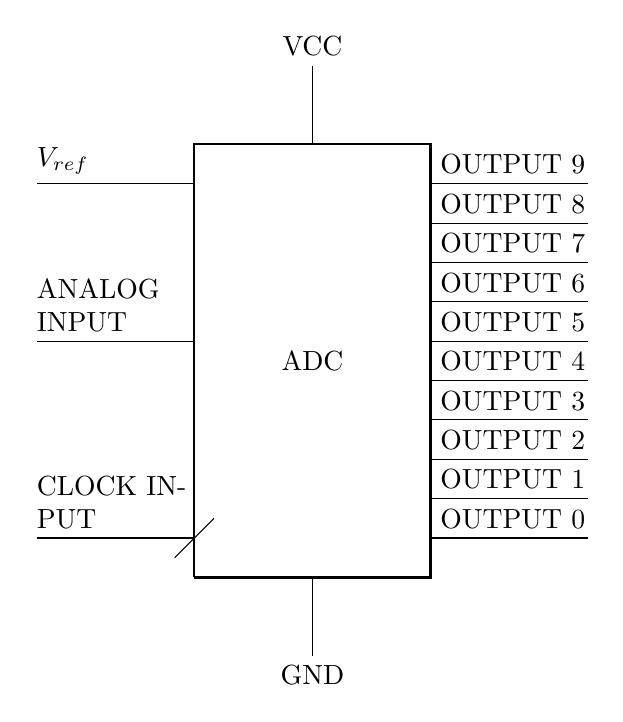
\begin{tikzpicture}
      \draw[thick] (0, 0) -- (0, 5.5) -- (3, 5.5) -- (3, 0) -- (0, 0);
      \draw (1.5, 2.5) node[right, above] {ADC};
      \draw (1.5, 5.5) -- (1.5, 6.5) node[right, above] {VCC};
      \draw (1.5, 0) -- (1.5, -1) node[right, below] {GND};
      \draw (-2, 5.0)
      -- (-1, 5.0) node[left, above, text width=2cm] {$V_{ref}$}
      -- (0, 5.0);
      \draw (0, 3.00)
      -- (-1, 3.00) node[left, above, text width=2cm] {ANALOG INPUT}
      -- (-2, 3.00);
      \draw (-2, 0.5)
      -- (-1, 0.5) node[left, above, text width=2cm] {CLOCK INPUT}
      -- (0, 0.5);
      \draw(-0.25, 0.25) -- (0.25, 0.75);
      \foreach \n/\y in {0/0.5, 1/1.0, 2/1.5, 3/2.0, 4/2.5, 5/3.0, 6/3.5, 7/4.0, 8/4.5, 9/5.0} {
        \draw (3, \y) node[anchor=south west] {OUTPUT \n} -- (5, \y);
      };
    \end{tikzpicture}
    \caption{\figureCaption}
    \label{fig:adc-schematics}
  \end{figure}
}

\newcommand{\figureAnalogSignalExample}[1]{
  \begin{figure}[ht]
    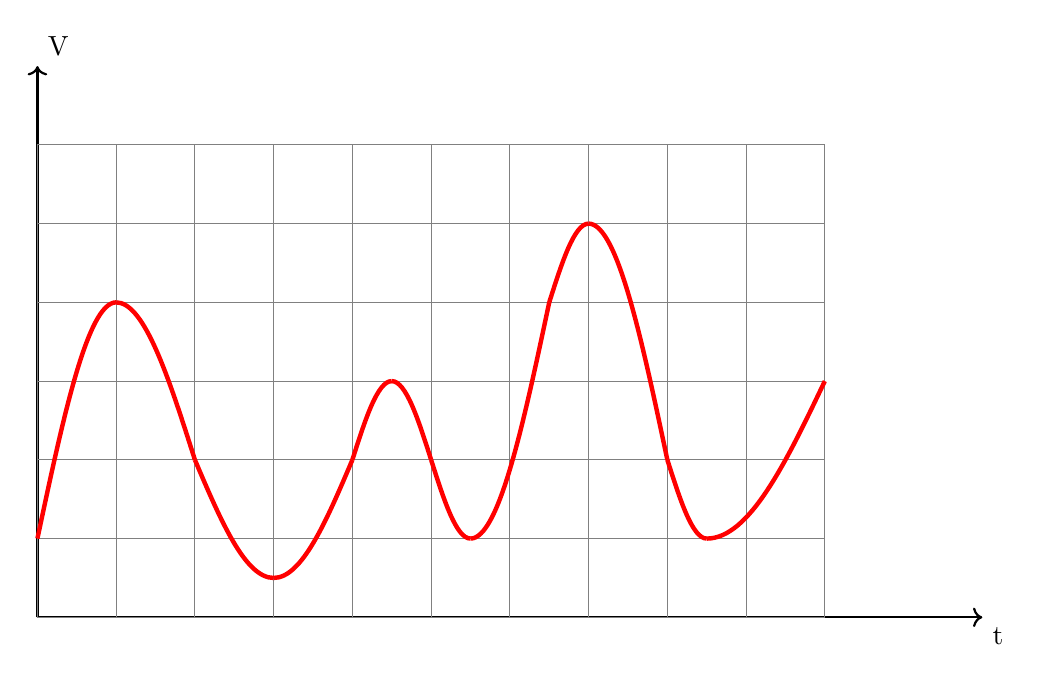
\begin{tikzpicture}
      \draw[thick, ->] (0, 0) -- (12, 0) node[anchor=north west] {t};
      \draw[thick, ->] (0, 0) -- (0,  7) node[anchor=south west] {V};
      \draw[gray] (0, 0) grid (10, 6);
      \draw[ultra thick, red] (0,1)   sin (1,4);
      \draw[ultra thick, red] (1,4)   cos (2,2);
      \draw[ultra thick, red] (2,2)   sin (3,0.5);
      \draw[ultra thick, red] (3,0.5) cos (4,2);
      \draw[ultra thick, red] (4,2)   sin (4.5,3);
      \draw[ultra thick, red] (4.5,3) cos (5,2);
      \draw[ultra thick, red] (5,2)   sin (5.5,1);
      \draw[ultra thick, red] (5.5,1) cos (6.5,4);
      \draw[ultra thick, red] (6.5,4) sin (7,5);
      \draw[ultra thick, red] (7,5)   cos (8,2);
      \draw[ultra thick, red] (8,2)   sin (8.5,1);
      \draw[ultra thick, red] (8.5,1) cos (10, 3);
    \end{tikzpicture}
    \caption{#1}
    \label{fig:adc-analog-signal-example}
  \end{figure}
}

\newcommand{\figureDigitalSignalExample}[1]{
  \begin{figure}[ht]
    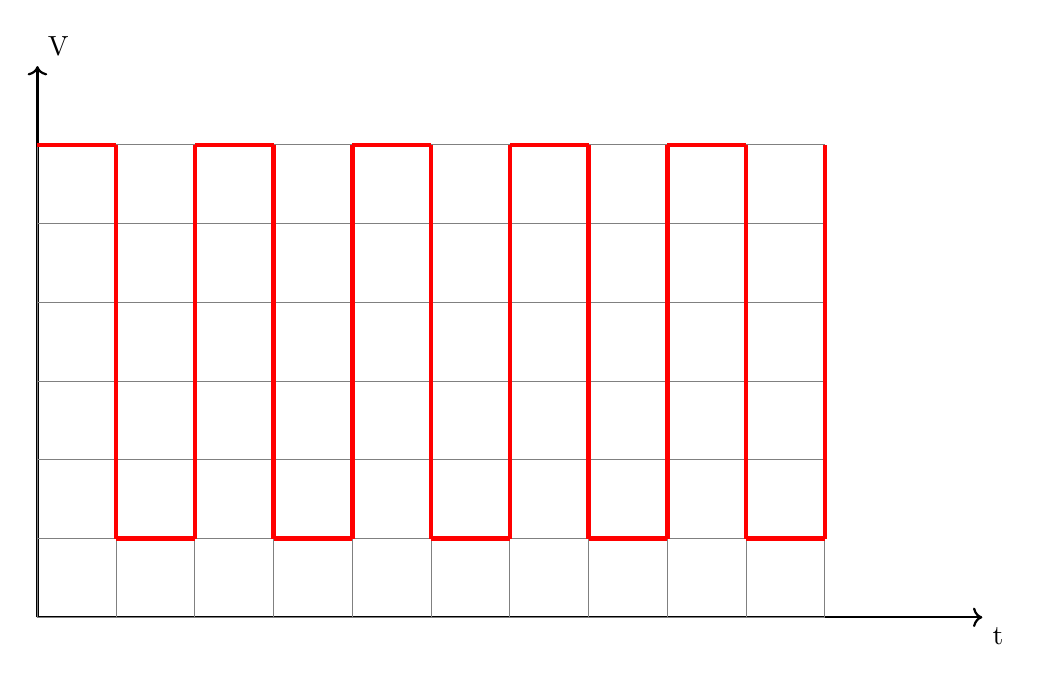
\begin{tikzpicture}
      \draw[thick, ->] (0, 0) -- (12, 0) node[anchor=north west] {t};
      \draw[thick, ->] (0, 0) -- (0,  7) node[anchor=south west] {V};
      \draw[gray] (0, 0) grid (10, 6);
      \foreach \x in {0, 2, ..., 8} {
        \draw[ultra thick, red] (\x, 6) -- (\x + 1, 6);
        \draw[ultra thick, red] (\x + 1, 6) -- (\x + 1, 1);
        \draw[ultra thick, red] (\x + 1, 1) -- (\x + 2, 1);
        \draw[ultra thick, red] (\x + 2, 1) -- (\x + 2, 6);
      }
    \end{tikzpicture}
    \caption{#1}
    \label{fig:adc-digital-signal-example}
  \end{figure}
}

\newcommand{\figureBlinkinLEDGraph}[1]{
  \def\lang{\detokenize{#1}}
  \def\langRu{\detokenize{ru}}
  \def\langEn{en}
  \def\figureCaption{XXX: No translation.}
  \ifx \lang\langRu
  \def\figureCaption{
    Графическое отображение сигнала, меняющегося во времени, на цифровом
    порту.
  }
  \fi
  \if \lang\langEn
  \def\figureCaption{
    Graphical representation of a signal in relation to the time on a
    digital port.
  }
  \fi
  \begin{figure}[ht]
    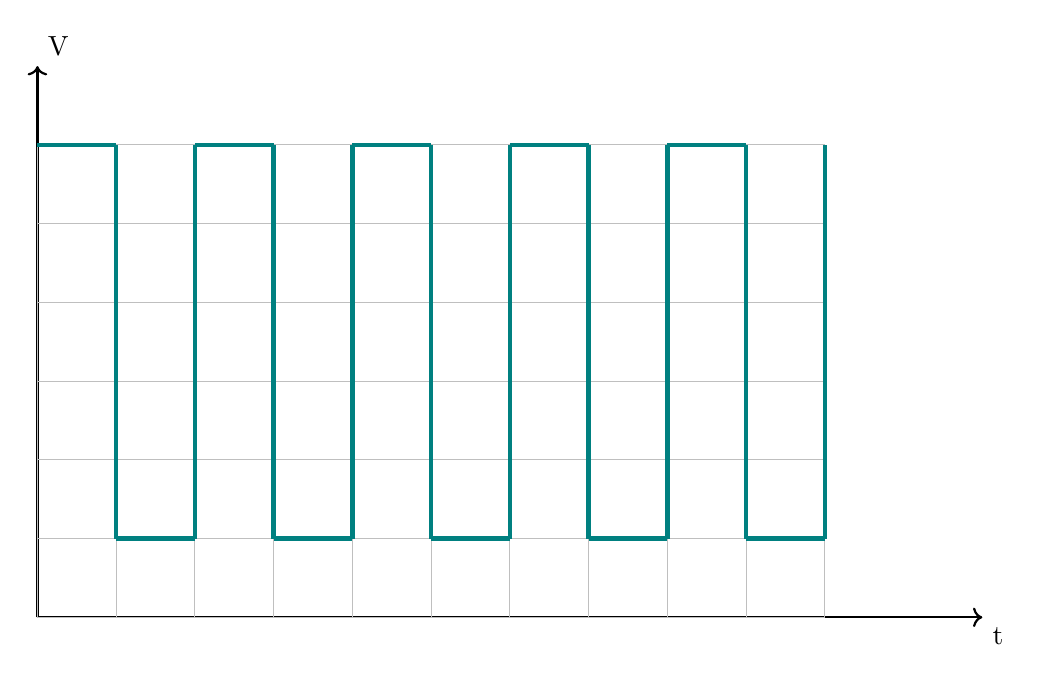
\begin{tikzpicture}
      \draw[thick, ->] (0, 0) -- (12, 0) node[anchor=north west] {t};
      \draw[thick, ->] (0, 0) -- (0,  7) node[anchor=south west] {V};
      \draw[lightgray] (0, 0) grid (10, 6);
      \foreach \x in {0, 2, ..., 8} {
        \draw[ultra thick, teal] (\x, 6) -- (\x + 1, 6);
        \draw[ultra thick, teal] (\x + 1, 6) -- (\x + 1, 1);
        \draw[ultra thick, teal] (\x + 1, 1) -- (\x + 2, 1);
        \draw[ultra thick, teal] (\x + 2, 1) -- (\x + 2, 6);
      }
    \end{tikzpicture}
    \caption{\figureCaption}
    \label{fig:blinking-led-graph}
  \end{figure}
}

\newcommand{\figureMusicSixBars}[1]{
  \begin{tikzpicture}
    \draw[thick, ->] (0, 0.5) -- (12, 0.5) node[anchor=north west] {t};
    \foreach \x/\n in {0/1, 2/2, 4/3, 6/4, 8/5, 10/6} {
      \draw (\x, 0) -- (\x, 1) -- (\x, 1) node[midway, above] {\n};
    };
    \label{fig:music-six-bar}
  \end{tikzpicture}
}

\newcommand{\figureMusicSixBarsFourFour}[1]{
  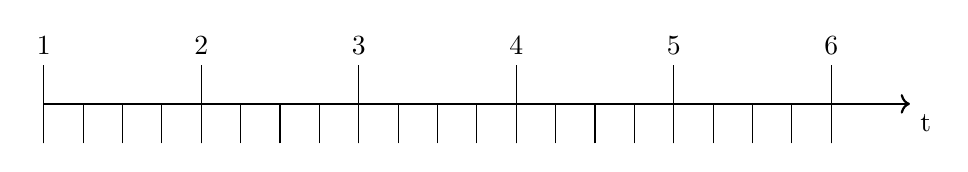
\begin{tikzpicture}
    \draw[thick, ->] (0, 0.5) -- (11, 0.5) node[anchor=north west] {t};
    \foreach \x/\n in {0/1, 2/2, 4/3, 6/4, 8/5, 10/6} {
      \draw (\x, 0) -- (\x, 1) -- (\x, 1) node[midway, above] {\n};
    };

    \foreach \x/\n in {0, 0.5, ..., 10} {
      \draw (\x, 0) -- (\x, 0.5);
    };
  \end{tikzpicture}
}

\newcommand{\figureMusicBarFourFour}[1]{
  \begin{tikzpicture}
    \draw[thick] (0, 0.5) -- (8, 0.5) node[anchor=north west] {t};
    \foreach \x/\n in {0/1, 8/2} {
      \draw (\x, 0) -- (\x, 1)  -- (\x, 1) node[midway, above] {\n};
    };

    \foreach \x in {0, 2, ..., 6} {
      \draw (\x, 0) -- (\x, 0.5) node[pos=0.25, right] {$ \frac{1}{4} $};
    };
  \end{tikzpicture}
}

\newcommand{\figureMusicBarFourFourWithFrequencies}[1]{
  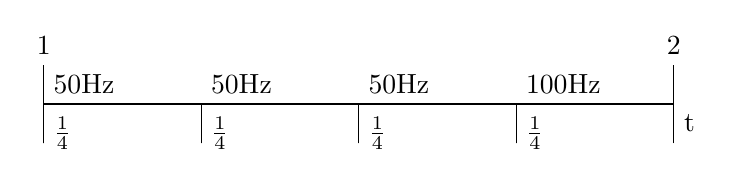
\begin{tikzpicture}
    \draw[thick] (0, 0.5) -- (8, 0.5) node[anchor=north west] {t};
    \foreach \x/\n in {0/1, 8/2} {
      \draw (\x, 0) -- (\x, 1) -- (\x, 1) node[midway, above] {\n};
    };

    \foreach \x in {0, 2, ..., 6} {
      \draw (\x, 0) -- (\x, 0.5) node[pos=0.25, right] {$ \frac{1}{4} $};
    };

    \foreach \x/\freq in {0/50, 2/50, 4/50, 6/100} {
      \draw (\x, 0) -- (\x, 0.5) node[pos=1.5, right] {\freq Hz};
    };
  \end{tikzpicture}
}

\newcommand{\figureMusicWeWillRockYouSimplified}[1]{
  \def\lang{\detokenize{#1}}
  \def\langRu{\detokenize{ru}}
  \def\langEn{en}
  \def\figureCaption{XXX: No translation.}
  \ifx \lang\langRu
  \def\figureHzUnit{Гц}
  \def\figureCaption{
    Ритм мелодии ``We Will Rock You'' группы Queen (упрощенная версия.)
  }
  \fi
  \if \lang\langEn
  \def\figureHzUnit{Hz}
  \def\figureCaption{
    The rhythm of the melody ``We Will Rock You'' by Queen (simplified
    version.)
  }
  \fi
  \begin{figure}[ht]
    \centering
    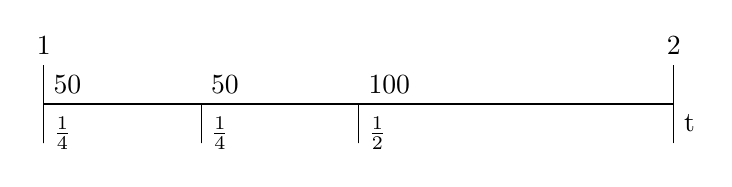
\begin{tikzpicture}
      \draw[thick] (0, 0.5) -- (8, 0.5) node[anchor=north west] {t};
      \foreach \x/\n in {0/1, 8/2} {
        \draw (\x, 0) -- (\x, 1) -- (\x, 1) node[midway, above] {\n};
      };

      \foreach \x in {0, 2} {
        \draw (\x, 0) -- (\x, 0.5) node[pos=0.25, right] {$ \frac{1}{4} $};
      };

      \draw (4, 0) -- (4, 0.5) node[pos=0.25, right] {$ \frac{1}{2} $};

      \foreach \x/\freq in {0/50, 2/50} {
        \draw (\x, 0) -- (\x, 0.5) node[pos=1.5, right] {\freq \figureHzUnit};
      };
      \draw (4, 0) -- (4, 0.5) node[pos=1.5, right] {100 \figureHzUnit};
    \end{tikzpicture}
    \caption{\figureCaption}
    \label{fig:queen-we-will-rock-you-rhythm-1}
  \end{figure}
}

\newcommand{\tableTwoDimensionalArray}[1]{
  \def\lang{\detokenize{#1}}
  \def\langRu{\detokenize{ru}}
  \def\langEn{\detokenize{en}}
  \def\tableFirstColumn{XXX: No translation.}
  \def\tableSecondColumn{XXX: No translation.}
  \def\tableCaption{XXX: No translation.}
  \ifx \lang\langRu
  \def\tableFirstColumn{
    № строки
  }
  \def\tableSecondColumn{
    № столбца
  }
  \def\tableCaption{
    Графическое отображение двумерного массива.
  }
  \fi
  \ifx \lang\langEn
  \def\tableFirstColumn{
    Row number
  }
  \def\tableSecondColumn{
    Column number
  }
  \def\tableCaption{
    Graphical representation of a two-dimensional array.
  }
  \fi
  \begin{table}[ht]
    \centering
    \begin{tabular}{r|l|l|l}
      \multicolumn{1}{l}{\tableFirstColumn}
      & \multicolumn{2}{l}{\tableSecondColumn}
      & \\
      \multicolumn{1}{l}{}         & \multicolumn{1}{l}{0} & \multicolumn{1}{l}{1} &   \\
      \cline{2-3}
      0                            & с4                    & 4                     &   \\
      \cline{2-3}
      1                            & с4                    & 4                     &   \\
      \cline{2-3}
      2                            & g4                    & 4                     &   \\
      \cline{2-3}
      3                            & g4                    & 4                     &   \\
      \cline{2-3}
      4                            & a4                    & 4                     &   \\
      \cline{2-3}
      5                            & a4                    & 4                     &   \\
      \cline{2-3}
      6                            & g4                    & 2                     &   \\
      \cline{2-3}
    \end{tabular}
    \caption{\tableCaption}
    \label{table:array-example-2}
  \end{table}
}

\newcommand{\tableMusicNoteLength}[1]{
  \def\lang{\detokenize{#1}}
  \def\langRu{\detokenize{ru}}
  \def\langEn{\detokenize{en}}
  \def\tableFirstColumn{XXX: No translation.}
  \def\tableSecondColumn{XXX: No translation.}
  \def\tableThirdColumn{XXX: No translation.}
  \def\tableCaption{XXX: No translation.}
  \def\tableWholeNote{XXX: No translation.}
  \def\tableHalfNote{XXX: No translation.}
  \def\tableQuarterNote{XXX: No translation.}
  \def\tableEighthNote{XXX: No translation.}
  \def\tableSixteenthNote{XXX: No translation.}
  \ifx \lang\langRu
  \def\tableFirstColumn{Начертание}
  \def\tableSecondColumn{Длительность}
  \def\tableThirdColumn{Название}
  \def\tableCaption{
    Некоторые возможные длительности нот.
  }
  \def\tableWholeNote{Целая}
  \def\tableHalfNote{Половина}
  \def\tableQuarterNote{Четверть}
  \def\tableEighthNote{Восьмая}
  \def\tableSixteenthNote{Шестнадцатая}
  \fi
  \ifx \lang\langEn
  \def\tableFirstColumn{Symbol}
  \def\tableSecondColumn{Length}
  \def\tableThirdColumn{Title}
  \def\tableCaption{
    Some of the possible lengths of the musical sounds (notes.)
  }
  \def\tableWholeNote{Whole note}
  \def\tableHalfNote{Half-note}
  \def\tableQuarterNote{Quarter-note}
  \def\tableEighthNote{Eighth-note}
  \def\tableSixteenthNote{Sixteenth-note}
  \fi

  \begin{table}[ht]
    \centering
    \def\arraystretch{2.5}%
    \begin{tabular}{|m{3cm}|m{4cm}|m{3.5cm}|}
      \hline
      \textbf{\tableFirstColumn}
      & \textbf{\tableSecondColumn}
      & \textbf{\tableThirdColumn} \\
      \hline
      {\Large \wholeNote} & {\Large $\frac{1}{1}$} & \tableWholeNote \\[2ex]
      \hline
      {\Large \halfNote}      & {\Large $\frac{1}{2}$}  & \tableHalfNote \\[2ex]
      \hline
      {\Large \quarterNote}   & {\Large $\frac{1}{4}$}  & \tableQuarterNote \\[2ex]
      \hline
      {\Large \eighthNote}    & {\Large $\frac{1}{8}$}  & \tableEighthNote \\[2ex]
      \hline
      {\Large \sixteenthNote} & {\Large $\frac{1}{16}$} & \tableSixteenthNote \\[2ex]
      \hline
    \end{tabular}
    \caption{\tableCaption}
    \label{table:music-notes-legths}
  \end{table}
}

\newcommand{\figureMusicTwinkleTwinkleLittleStar}[1]{
  \def\lang{\detokenize{#1}}
  \def\langRu{\detokenize{ru}}
  \def\langEn{\detokenize{en}}
  \def\figureCaption{XXX: No translation.}
  \ifx \lang\langRu
  \def\figureCaption{
    Мелодия ``Twinkle, Twinkle, Little Star''.
  }
  \fi
  \ifx \lang\langEn
  \def\figureCaption{
    ``Twinkle, Twinkle, Little Star'' melody.
  }
  \fi
  \begin{figure}[ht]
    \centering
    \begin{lilypond}
      \relative c' {
        \numericTimeSignature
        \time 4/4
        c4 c g' g
        a a g2
        f4 f e e
        d d c2
        g'4 g f f
        e e d2
        g4 g f f
        e e d2
        c4 c g' g
        a a g2
        f4 f e e
        d d c2
      }
      \layout {
        indent = 0\mm
        line-width = 100\mm
        ragged-last = ##t
      }
    \end{lilypond}
    \caption{\figureCaption}
    \label{fig:sound-fig-3}
  \end{figure}
}


\counterwithin{listing}{section}

\newgetenv[\REPRODUCIBILITY]{REPRODUCIBILITY}%
\newgetenv[\RANDOMSEED]{RANDOMSEED}

\ifdefstring{\REPRODUCIBILITY}{yes}{%
  \ifthenelse{\equal{\RANDOMSEED}{}}%
  {%
    \typeout{Setting the random seed to a fixed value.}%
    \pgfmathsetseed{\number42}%
  }{%
    \typeout{Setting the random seed to a \RANDOMSEED .}%
    \pgfmathsetseed{\number\RANDOMSEED}%
  }%
}{}

%%%%%%%%%%%%%%%%%%%%%%%%%%%%%%%%%%%%%%%%%%%%%%%%%%%%%%%%%%%%%%%%%%%%%%%%%%%%%%%%
\title{Science, Programming, Art and Radioelectronics Club\\(SPARC)}
\author{Artyom ``avp'' Poptsov\\\href{https://memory-heap.org}{memory-heap.org}}
\input{out/src/en/version.tex}

\begin{document}

\maketitle

\tableofcontents

%%%%%%%%%%%%%%%%%%%%%%%%%%%%%%%%%%%%%%%%%%%%%%%%%%%%%%%%%%%%%%%%%%%%%%%%%%%%%%%%
\chapter*{Introduction}
\addcontentsline{toc}{chapter}{Introduction}

%% TODO:

\subfile{sections/introduction.tex}

%%%%%%%%%%%%%%%%%%%%%%%%%%%%%%%%%%%%%%%%%%%%%%%%%%%%%%%%%%%%%%%%%%%%%%%%%%%%%%%%
\chapter{Electronics}
\label{chapter:electronics}

%% TODO:
\subfile{sections/electronics-introduction.tex}
\subfile{sections/electronics-voltage}
\subfile{sections/electronics-circuits.tex}
\subfile{sections/electronics-potential-difference}
\subfile{sections/electronics-resistance}
\subfile{sections/electronics-building-circuits}

%%%%%%%%%%%%%%%%%%%%%%%%%%%%%%%%%%%%%%%%%%%%%%%%%%%%%%%%%%%%%%%%%%%%%%%%%%%%%%%%
\chapter{Dialogues with a Computer}
\label{chapter:dialogues-with-computer}

\subfile{sections/dialogues-with-computer-title-image}
\subfile{sections/dialogues-with-computer-introduction}
\subfile{sections/dialogues-with-computer-algorithms}
\subfile{sections/dialogues-with-computer-arduino}
\subfile{sections/dialogues-with-computer-breadboard}
\subfile{sections/dialogues-with-computer-multimeter}

\newpage
\subfile{sections/dialogues-with-computer-arduino-ide}
\subfile{sections/dialogues-with-computer-program-structure}
\subfile{sections/dialogues-with-computer-memory}
\subfile{sections/dialogues-with-computer-control-flow}
\subfile{sections/dialogues-with-computer-wokwi}

%%%%%%%%%%%%%%%%%%%%%%%%%%%%%%%%%%%%%%%%%%%%%%%%%%%%%%%%%%%%%%%%%%%%%%%%%%%%%%%%
\chapter{White noise}
\label{chapter:white-noise}

\subfile{sections/white-noise-introduction}
\subfile{sections/white-noise-signal-types}
\subfile{sections/white-noise-serial-port}
\subfile{sections/white-noise-analog-ports}
\subfile{sections/white-noise-adc}

%%%%%%%%%%%%%%%%%%%%%%%%%%%%%%%%%%%%%%%%%%%%%%%%%%%%%%%%%%%%%%%%%%%%%%%%%%%%%%%%
\chapter{Pulse-Width Modulation}
\label{chapter:pwm}

\subfile{sections/pwm-intro}
\subfile{sections/pwm-wavelength}
\subfile{sections/pwm-duty-cycle}
\subfile{sections/pwm-tasks}

%%%%%%%%%%%%%%%%%%%%%%%%%%%%%%%%%%%%%%%%%%%%%%%%%%%%%%%%%%%%%%%%%%%%%%%%%%%%%%%%
\chapter{Music and Technology Synthesis}
\label{chapter:music-and-technology-synthesis}

\subfile{sections/music-and-technology-synthesis-sound}
\subfile{sections/music-and-technology-synthesis-speaker}
\subfile{sections/music-and-technology-synthesis-rhythm}
\subfile{sections/music-and-technology-synthesis-harmony}
\subfile{sections/music-and-technology-synthesis-octave-system}
\subfile{sections/music-and-technology-synthesis-simple-melodies}
\subfile{sections/music-and-technology-synthesis-arrays}
\subfile{sections/music-and-technology-synthesis-two-dimensional-arrays}
\subfile{sections/music-and-technology-synthesis-staff}
\subfile{sections/music-and-technology-synthesis-rest}
\subfile{sections/music-and-technology-synthesis-dotted-notes}
\subfile{sections/music-and-technology-synthesis-flats-and-sharps}
\subfile{sections/music-and-technology-synthesis-time-signature}
\subfile{sections/music-and-technology-synthesis-bass-clef}
\subfile{sections/music-and-technology-synthesis-music-band}

%%%%%%%%%%%%%%%%%%%%%%%%%%%%%%%%%%%%%%%%%%%%%%%%%%%%%%%%%%%%%%%%%%%%%%%%%%%%%%%%
%% \chapter{Computer Language}
%% \label{chapter:computer-language}

%% TODO:

%%%%%%%%%%%%%%%%%%%%%%%%%%%%%%%%%%%%%%%%%%%%%%%%%%%%%%%%%%%%%%%%%%%%%%%%%%%%%%%%
%% \chapter{Game Development}
%% \label{chapter:game-development}

%% TODO:

%%%%%%%%%%%%%%%%%%%%%%%%%%%%%%%%%%%%%%%%%%%%%%%%%%%%%%%%%%%%%%%%%%%%%%%%%%%%%%%%
\addcontentsline{toc}{chapter}{Index}
\printindex

%%%%%%%%%%%%%%%%%%%%%%%%%%%%%%%%%%%%%%%%%%%%%%%%%%%%%%%%%%%%%%%%%%%%%%%%%%%%%%%%
\addcontentsline{toc}{chapter}{Glossary}
\printglossaries

%%%%%%%%%%%%%%%%%%%%%%%%%%%%%%%%%%%%%%%%%%%%%%%%%%%%%%%%%%%%%%%%%%%%%%%%%%%%%%%%
\addcontentsline{toc}{chapter}{Code listings}
\renewcommand\listoflistingscaption{Code listings}
\listoflistings

%%%%%%%%%%%%%%%%%%%%%%%%%%%%%%%%%%%%%%%%%%%%%%%%%%%%%%%%%%%%%%%%%%%%%%%%%%%%%%%%
\printbibliography[heading=bibintoc, title={Bibliography}]

%%%%%%%%%%%%%%%%%%%%%%%%%%%%%%%%%%%%%%%%%%%%%%%%%%%%%%%%%%%%%%%%%%%%%%%%%%%%%%%%
\appendix

\subfile{sections/appendix-octaves}
\subfile{sections/appendix-prostokvashino-score}
\subfile{sections/appendix-twinkle-twinkle-little-star-01}
\subfile{sections/appendix-twinkle-twinkle-little-star-02}

\end{document}
